\documentclass[10pt]{article}
\usepackage[T1]{fontenc} 
\usepackage{bbold}
\usepackage{tikz, lipsum,lmodern}
\usepackage{hyperref}

\usepackage{nicematrix,tikz}
\usepackage[tmargin=2cm,rmargin=1in,lmargin=1in,margin=0.85in,bmargin=2cm,footskip=.2in]{geometry}
\usepackage{amsmath,amsfonts,amsthm,amssymb,mathtools}
%\usepackage{authblk}
\usepackage{nameref}
\usepackage{multicol,array}
\usepackage{tikz-cd}
\usepackage[ruled,vlined,linesnumbered]{algorithm2e}
\usepackage{pdfpages}


\title{Report - Praxisblatt 1}
\author{Malte A. Weyrich \& Jan P. Hummel}
\begin{document}

\maketitle
\section*{Disclaimer}
    Alle Werte die in diesem Report vorgestellt werden, wurden auf einem \textit{Lenovo-ThinkPad-Gen-1} Rechner mit
    folgender Hardware \textit{AMD® Ryzen 7 pro 4750u with radeon graphics × 16; Memory: 16.0 GB} erhoben. 
    Die Dokumentation zur \textit{usage} der \textit{SMSS JAR} ist auf dem \textbf{README.md} des folgenden
    \textit{GitHub Repository:} \url{http://https://github.com/github4touchdouble/smss} zu finden.

\section{Aufgabe}
    \subsection{Naive Approaches}
    Der \textit{naive} Ansatz verfolgt eine recht simple Strategie, um alle Segmente in dem
    Vector C zu identifizieren und die Summe zu bilden. Vom Arbeitsspeicher her ist dieser Ansatz
    sehr schonend, da die Variablen ( wie z.B. \textit{maxscore, l, r} usw.) immer einzeln gespeichert werden
    und gegebenen Falls überschrieben werden. Jedoch liegt der gro\ss e Nachteil bei der Laufzeit, welche sich
    folgender ma\ss en beschreiben lässt:
    \[
        \frac{n^{3}+3n^{2}+2n}{6} 
    \]
    Der \textit{rekursive} Ansatz spart sich einige Schritte in der Berechnung, jedoch bleibt der dominante Term weiterhin
    $n^{3}$:
    \[
       \frac{n^{3}-n}{6}  
    .\]
    Zudem leidet der Stack unter den polynomiell steigenden Funktionsaufrufen, was bereits bei 
    kleinen Eingaben zu Problemen führt. Man könnte also argumentieren, dass obwohl der \textit{rekursive}
    Ansatz auf dem Papier etwas effizienter ist, für gro\ss e Eingaben immer noch der \textit{naive} Ansatz
    am realistischen ist. Beide Algorithmen sind zeitlich eingeschränkt, vor allem ist aber der 
    \textit{rekursive} Ansatz klar limitiert (vom Arbeitsspeicher) was die Eingabegrö\ss e $n$ an geht.
    In Abbildung \ref{fig:naiv_vs_rec} ist die Laufzeit in Sekunden beider Ansätze gegen die Eingabelänge $n$ grafisch dargestellt:

    \begin{figure}[ht]
        \centering
        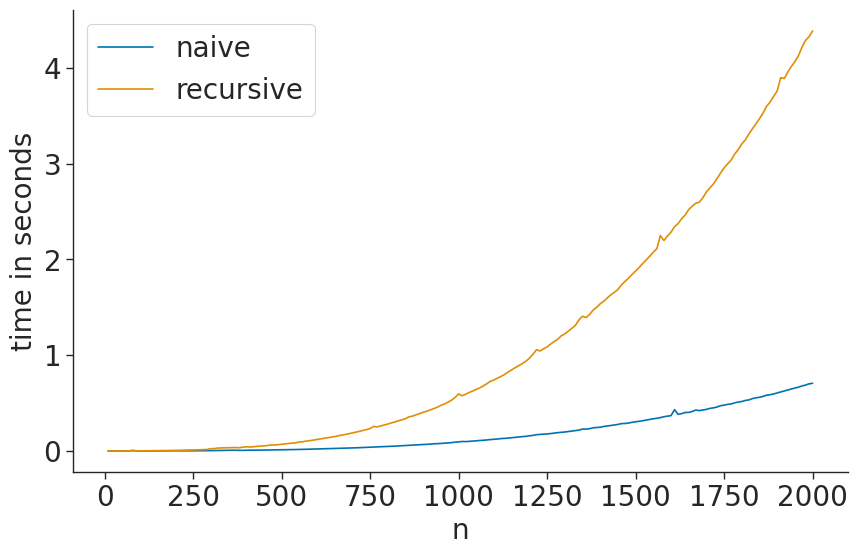
\includegraphics[width=0.45\textwidth]{../naive_vs_rec_times.png}
        \caption{\textit{Naive} algorithm versus \textit{recursive} solution.}
        \label{fig:naiv_vs_rec}
    \end{figure}

        \newpage
    Wie sich herausstellt, skaliert der \textit{naive} Ansatz auf der gegebene Hardware besser als der \textit{rekursive} Ansatz.
    Das liegt wahrscheinlich an den vielen rekursiven Aufrufen, die alle ebenfalls Zeit kosten und daran, wie Java 
    intern mit den Rekursionsaufrufen umgeht. 

    \subsection{Dynamic Programming}\label{sec:dynamic}
    Der \textit{dynamic programming} Ansatz bedient sich eines Arrays, welches bereits berechnete Ergebnisse zwischenspeichert und somit
    redundante Berechnungen verhindert. Somit verbessert sich die Laufzeit stark verglichen zu den oberen Ansätzen:

    \[
        \frac{n^{2}+n}{2} 
    .\]

    Jedoch bu\ss t dieser Ansatz damit ein, dass der Speicherplatzbedarf quadratisch steigt und das Array jedes mal 
    initialisiert werden muss, was wiederum Zeit benötigt. Zudem ist die Nutzung des Arrays nicht optimal. Es wird jeweils nur die 
    Hälfte des reservierten Speicherplatzes tatsächlich genutzt. In \ref{sec:2c} wird diese Optimierung 
    umgesetzt.

    \subsection{Divide and Conquer \& Optimal Solution}
   Der \textit{divide and conquer} hat eine Komplexität von ....
       TODO JAAAN



       Der \textit{optimale} Ansatz löst das Problem in linearer Zeit $\mathcal{O}(n)$. 
   Genau wie im \textit{naiven} Ansatz werden hier keine zusätzlichen Datenstrukturen verwendet,
   lediglich werden einzelne Integers gespeichert und überschreiben. Demnach ist der \textit{optimale}
   Ansatz auch bezogen auf den Arbeitsspeicher sehr effizient. 



\section{Aufgabe}

\subsection{2a - SMSS}\label{sec:2a}
Wir erweitern den optimalen Ansatz, indem wir jedes gefundene \textit{segment} in einer \textit{ArrayList< ArrayList<int[3]> >} abspeichern.
Die äu\ss ere Liste initialisiert für jeden neuen \textit{max\_score} der gefunden wurde eine neue innere Liste. Diese innere
Liste wird so lange mit gleichwertigen \textit{segmenten} befüllt, bis ein \textit{segment} gefunden wurde, mit einen grö\ss erem
\textit{max\_score}. So ist die Liste von links nach rechts aufsteigend nach \textit{max\_score} sortiert (d.h. die letzte innere Liste beinhaltet alle \textit{MSS}).
Am Ende wird einmal über die am \textit{Endindex} stehende Liste in $\mathcal{O}(n)$ iteriert, um die tatsächlichen non overlapping
\textit{MSS} in einer finale Liste zu speichern.

Folgende Fälle werden abgedeckt: \\
\begin{verbatim} 
   CASE 1:
   1: ---+===+-----------
   2: ---+=====+---------
\end{verbatim}
Hier darf das $segment_{2}$ nicht ausgegeben werden, da $segment_{1} \subseteq segment_2$. Also merken wir uns
jeweils den Start- und Endindex des letzten \textit{segments}. So können wir die letzten Indizes mit den 
momentanen vergleichen und \textbf{CASE 1} abfangen. 

\begin{verbatim}
   CASE 2:
   1: ---+=====+---------
   2: ---+===+-----------
\end{verbatim}
\textbf{CASE 2} ist nicht möglich, da $segment_{2}$ vor $segment_{1}$ in der Liste abgespeichert ist.
Der Algorithmus ist so konzipiert, dass er wie bei \textbf{CASE 1} erst das kürzere $segment_{1}$ findet und dann das
längere $segment_{2}$. Also müssen wir uns nicht um \textbf{CASE 2} kümmern.
\begin{verbatim}
   CASE 3:
   1: -----+=+-----------
   2: ---+=====+---------

   CASE 4
   1: ---+=====+---------
   2: -----+=+-----------
\end{verbatim}
\textbf{CASE 3 \& 4} Sind ebenfalls nicht möglich, da \textit{MSS} entweder den gleichen Start- oder Endindex haben.

\begin{verbatim} 
   CASE 5:
   1: -----+===+---------
   2: ---+=====+---------
\end{verbatim}
Hier wird sich in der \textit{i-ten} Iteration die Start- und Endindizes von $segment_{1}$ gemerkt
und demnach das $segment_{2}$ in der \textit{i+1-ten} Iteration nicht dem Endresultat hinzugefügt,
da der Endindex von $segment_2 \not >$  Endindex von $segment_1$.

\subsection{2b - SMSS mit minimaler Länge}\label{sec:2b}
Wir verwenden den Algorithmus aus \ref{sec:2a}, um alle SMSS zu finden. 
Unser Ziel ist es, aus der Ergebnismenge von \ref{sec:2a} die SMSS mit minimaler Länge zu ermitteln. 
Hierbei interessieren wir uns für die Länge jeder Sequenz in der Ergebnismenge sowie für 
die minimale Länge aller Sequenzen aus \ref{sec:2a}).
Der Algorithmus durchläuft die Ergebnismenge aus \ref{sec:2a} in linearer Zeitkomplexität $\mathcal{O}(n)$ 
und bestimmt für jede Sequenz die Länge anhand der Differenz zwischen ihrem Start- und Endindex in 
konstanter Zeit $\mathcal{O}(1)$. Während dieses Prozesses wird fortlaufend überprüft, 
ob die aktuelle Sequenz die bisher kürzeste ist, was ebenfalls in konstanter Zeit erfolgt $\mathcal{O}(i)$. 
Sequenzen gleicher Länge werden in einer Liste zusammengefasst, wobei die Sequenzlängen als Schlüssel 
in einer \textit{HashMap} dienen. Dadurch ist ein schneller Zugriff gewährleistet, 
da der Zugriffsschlüssel (die Sequenzlänge) bekannt ist, was zu einer angenäherten Zugriffszeit von 
$\mathcal{O}(1)$ führ.
Am Ende des Durchlaufs ist die minimale Sequenzlänge bekannt, und die Liste der Sequenzen mit dieser 
Länge kann durch einen Lesezugriff auf die \textit{HashMap} als Ergebnismenge extrahiert werden.
Mit zunehmender Größe der Eingabemenge steigt die Laufzeit von 2b) linear an. 
Jedes Element wird einmal gespeichert, wodurch auch die Speicherbelastung proportional mit der 
Größe der Eingabe wächst.

Anzumerken ist, dass die tatsächliche Laufzeit dieses Ansatzes auf der Konzeption und Implementierung 
von \ref{sec:2a} abhängt. 
Eine Laufzeitkomplexität von \ref{sec:2a} in $\mathcal{O}(n)$ ist vorausgesetzt, sodass die 
Laufzeitkomplexität von 2b) in $\mathcal{O}(n)$ liegt, da 2b) die Ergebnismenge 
aus \ref{sec:2a} als Eingabe verarbeitet.
Die Sortierung der Ergebnismenge aus \ref{sec:2a} spielt keine Rolle, da allein aus der Kenntnis der minimalen 
Sequenzlänge nicht automatisch die Anzahl oder die Indexpositionen der SMSS mit minimaler Länge in 
der Ergebnismenge aus \ref{sec:2a} folgen. 
Selbst wenn die Ergebnismenge nach Sequenzlänge aufsteigend sortiert ist, wird der beschriebene 
Algorithmus 2b) angewendet. Lediglich könnte die Iteration vorzeitig abgebrochen werden, 
wenn für ein Element die berechnete Sequenzlänge größer als die bisher bekannte minimale Länge ist. 
In diesem Fall wäre aufgrund der Sortierung sichergestellt, dass alle SMSS mit minimaler 
Länge gefunden wurden. Der Algorithmus 2b) müsste im Falle einer sortierten Ergebnismenge leicht 
angepasst werden, um diese Bedingung zu überprüfen und die Iteration gegebenenfalls abzubrechen.

\subsection{2c - Alle MSS}\label{sec:2c}

Für die 2c haben wir unseren ursprünglichen Ansatz nicht weiter verwendet. Der \textit{optimale Algorithmus} ist in sich selbst so effizient,
dass er null Folgen am Anfang und am Ende von Segmenten direkt ignoriert. Wir haben uns also überlegt, welcher der anderen 
Algorithmen mit eine möglichst guten Laufzeit, diese Fälle auch betrachtet. Wir haben uns dazu entschieden 
den \textit{dynamic programming Algorithmus} zu erweitern. Dieser hat nämlich den Vorteil
bereits ohne Erweiterungen, alle Kombinationen von Teilintervallen zu betrachten. Insbesondere die Teilintervalle,
die der \textit{optimale Algorithmus} nicht in Betracht zieht. Im unteren Fallbeispiel sieht man, wie der \textit{optimale Algorithmus}
die Nullerpräfixe der MSS ignoriert:
\begin{verbatim}
Für Sequenz:            5 -5 9 -3 13 -5 5 -5 5
optimal             :   -----+=====+----------

tatsächliche MSS    :   -----+=====+----------
                        -----+==========+-----
                        -----+===============+
                        +==========+----------
                        +===============+-----
                        +====================+
\end{verbatim}

Der \textit{dynamic programming} Algorithmus betrachtet in dem oberen Beispiel alle der Teilfolgen. 
Also haben wir wieder wie in \ref{sec:2a} eine äu\ss ere Liste mit inneren Listen erstellt, und für jeden neuen \textit{maxscore} eine neue innere Liste
erstellt, die dann mit allen gleichwertigen Segmenten (also allen Segmenten mit demselben \textit{maxscore}) befüllt wird, bis ein grö\ss erer \textit{maxscore} gefunden wird.
So findet der \textit{2\_c Algorithmus} also definitiv alle MSS, denn wir wissen bereits, dass der \textit{dynamic programming} Ansatz korrekt ist und
alle Kombinationen in Betracht zieht. Jedoch bu\ss t dieser Ansatz bei der Speicherkomplexität ein, das \textit{int[][]} Array wächst 
zu einem gegebenen Eingabe Vektor mit Länge $n$ exponentiell: $n^{2}$. D.h. für gro\ss e Eingaben verbrauchen wir enorm viel
Speicherplatz. 
Wie bereits in \ref{sec:dynamic} gezeigt, benutzt der \textit{dynamic programming} Ansatz immer nur 
die Hälfte des Arrays. Allgemein hat das Array die folgende Form:

$$
    \begin{pNiceMatrix}[left-margin]
    \times & \times & \times & \times & \times \\
           & \times & \times & \times & \times \\
           &        & \times & \times & \times \\ 
    \Block{2-2}<\Huge>{0}
           &        &        & \times & \times \\
           &        &        &        & \times \\
    \CodeAfter
     \tikz \draw (2-|1) -| (3-|2) -| (4-|3) -| (5-|4) -| (6-|5) ;
    \end{pNiceMatrix}
$$

 Betrachten wir die jeweiligen Endzustände der Datenstruktur $S$ von Algorithmus \textit{2\_c} und der 
 Arbeitsspeicher schonenden Variante \textit{2\_c\_1}:

\begin{verbatim}
 Eingabe: v = {5, -5, 9, -3, 13, -5, 5, -5, 5}
 Array S[n][n] of Default Dynamic Programming (2_c) on v:
    0: [5 ,0 ,9 ,6 ,19,14,19,14,19]
    1: [0 ,-5,4 ,1 ,14,9 ,14,9 ,14]
    2: [0 ,0 ,9 ,6 ,19,14,19,14,19]
    3: [0 ,0 ,0 ,-3,10,5 ,10,5 ,10]
    4: [0 ,0 ,0 ,0 ,13,8 ,13,8 ,13]
    5: [0 ,0 ,0 ,0 ,0 ,-5,0 ,-5, 0]
    6: [0 ,0 ,0 ,0 ,0 ,0 ,5 , 0, 5]
    7: [0 ,0 ,0 ,0 ,0 ,0 ,0 ,-5, 0]
    8: [0 ,0 ,0 ,0 ,0 ,0 ,0 , 0, 5]
                               
 Max n on given Hardware: 30808:
 java -jar SMSS.jar --algorithms 2_c --size 30808
\end{verbatim}

\begin{verbatim}
 Eingabe: v = {5, -5, 9, -3, 13, -5, 5, -5, 5}
 ArrayList S containing int[] Arrays of Improved Dynamic Programming (2_c_1) on v:
    0: [5 ,0 ,9 ,6 ,19,14,19,14,19]
    1: [-5,4 ,1 ,14,9 ,14,9 ,14]
    2: [9 ,6 ,19,14,19,14,19]
    3: [-3,10,5 ,10,5 ,10]
    4: [13,8 ,13,8 ,13]
    5: [-5,0 ,-5,0]
    6: [5 ,0 ,5]
    7: [-5,0]
    8: [5]

 Max n on given Hardware: 44069:
 java -jar SMSS.jar --algorithms 2_c_1 --size 44069
\end{verbatim}

Der \textit{improved dynamic programming 2\_c\_1} hat keine Position in der 
Datenstruktur, die ungenutzt bleibt. Der verbesserte Ansatz schafft es $13261$ zusätzliche
Zahlen zu verarbeiten, also ein $\approx 43\%$ grö\ss eres $n$ als der \textit{default 2\_c Algorithmus} 
(*auf der gegebenen Hardware). An der Komplexität hat sich durch die Abänderungen nichts geändert.
In Abbildung \ref{fig:time_comp_2c} werden die zwei Ansätze in ihrer Laufzeit verglichen.
Die Spikes in der Abbildung entstehen durch die inkonsistente Geschwindigkeit bei der Array Initialisierung.


\begin{figure}[t]
    \centering
    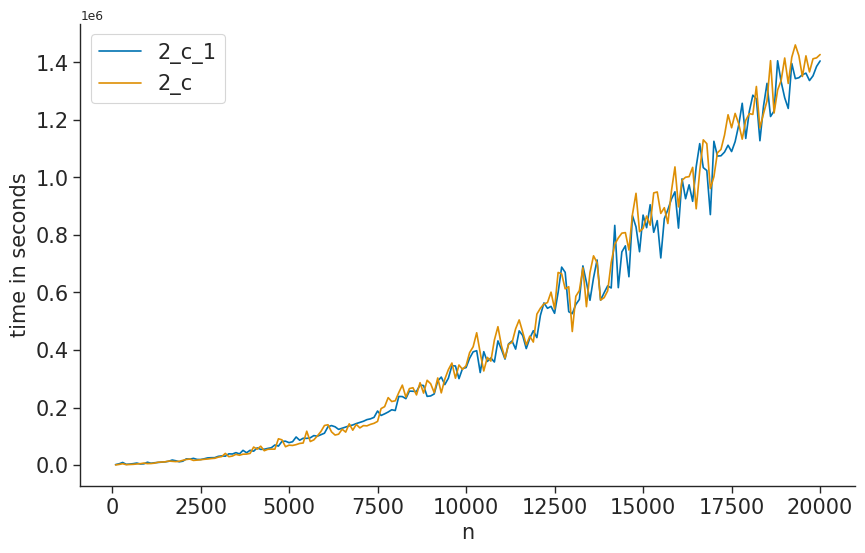
\includegraphics[width=0.8\textwidth]{../times_2c_20000.png}
    \caption{Ansatz 2\_c verglichen mit dem Arbeitsspeicher optimierten Ansatz 2\_c\_1}
    \label{fig:time_comp_2c}
\end{figure}

\section{Supplementary Material}


\begin{figure}[ht]
    \centering
    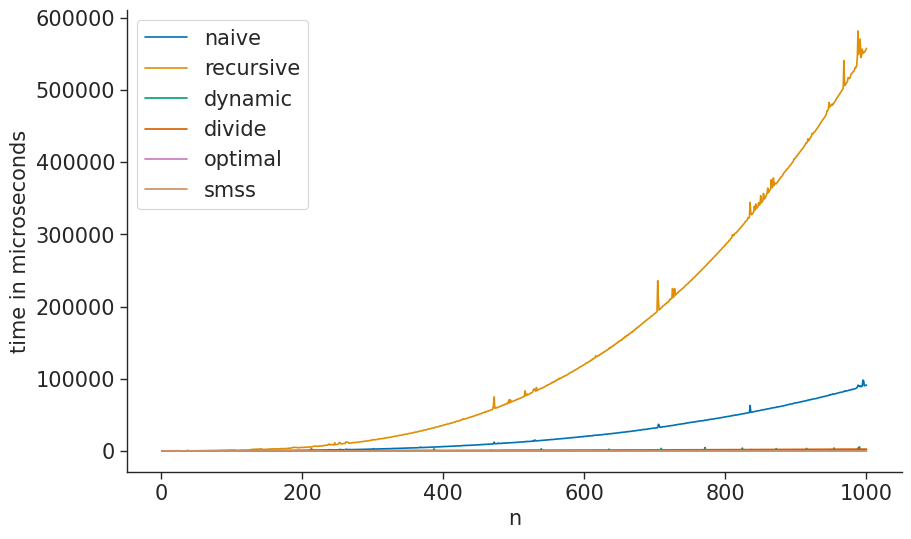
\includegraphics[width=0.8\textwidth]{../times_1000_all.png}
    \caption{Überblick aller Algorithmen für Eingabeintervall [1; 1000]}
    \label{fig:overview}
\end{figure}
\end{document}
